\section{Discussion and Future Work}
\label{sec:discussion}
In this section, we answer our research questions and discuss our interpretation of this result. We then highlight recommendations to practitioners using QS for collective decision making and highlight future directions for QS research.

\subsection{QS's effectiveness and its dual components}
In this study, we aim to examines how effectively QS captures participant preferences compared to Likert scale surveys at a pairwise level (RQ1) and understand whether QS requires both the quadratic cost function and a fixed budget to make it effective (RQ2). Our dual analysis comparing QS (votes and credit spent), Likert, UQS, and LS further supports that QS exhibits superior performance in preference elicitation compared to Likert Scale Surveys. Within ordinal preference prediction, QS shows a statistically significant but modest advantage over Likert scales, even QS with small budget. For preference intensity, QS performs better Likert scale surveys as the magnitude of preference differentials increases between options. Altogether, we demonstrated that QS better Likert overall should the survey designer aim to capture accurate individual preferences across multiple options under resource constraint scenarios for collective decision making.

With the added experiment in this study, our empirical findings demonstrates both the quadratic cost function and budget constraint constitute the effectiveness of QS mechanism. The removal of either component (as implemented in Unlimited QS or Linear Survey) results in diminished performance as discussed in~\Cref{sec:result_2}. Pragmatically, this result indicates that rather than applying LS for reduced cognitive load and ease of completion, further research should guide developers in designing systems that aids QS completion. Scientifically, the result raised our interest to understand why LS did not work as well.

% insert figure
\begin{figure}[h]
    \centering
    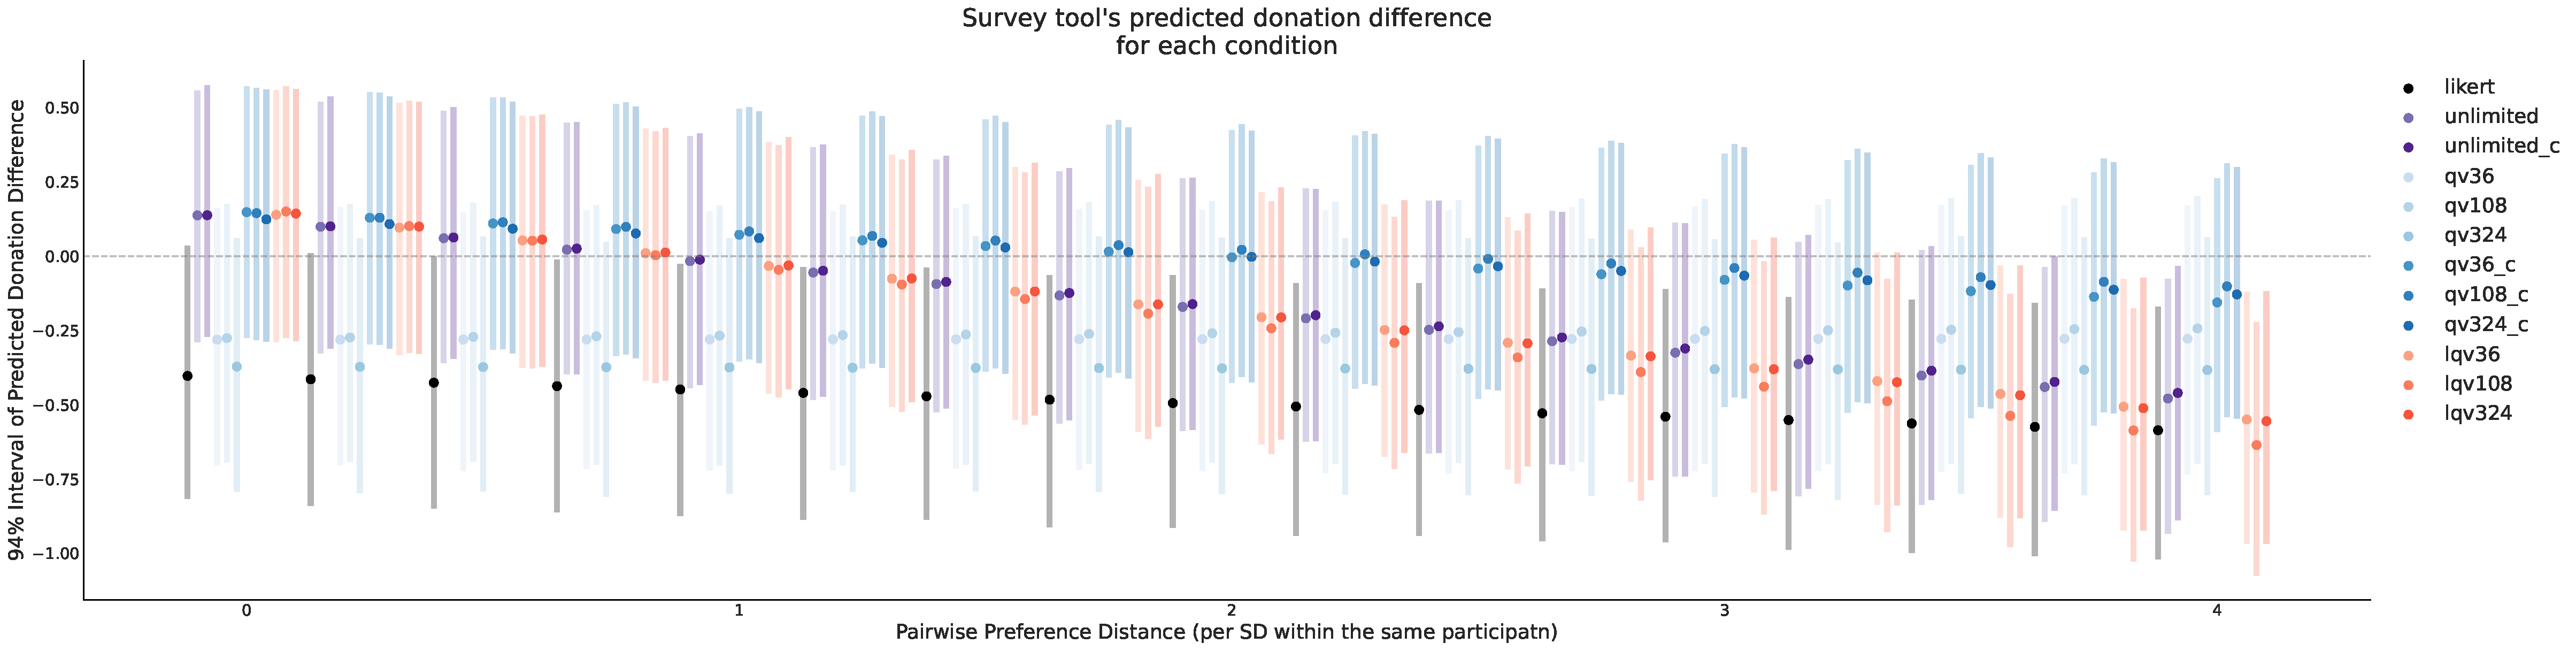
\includegraphics[width=\textwidth]{content/image/Predicted_Donation_Diff_Interval.pdf}
    \caption{Comparison of preference elicitation methods: QS, LS, UQS, and Linear Survey.}
    \label{fig:comparison}
\end{figure}

\subsection{Distortion in survey's `preference units'}
Among options, people have strong preferences between some pairs and less among others.~\Cref{fig:comparison} shows how different survey tools capture these pairwise differences. As discussed in Section~\ref{}, while QV credits remain reflective of individual's behavior, the stronger a participant treat a pairwise option across all options, the more LS response difference underestimates it. If we define a `preference unit' as each additional preference interval the participant expressed (i.e., an additional vote, or selecting the next preference interval), this result means that individuals `perceived' less preference increases per additional preference unit, hence the underestimation. This behavior mirrors psychophysics' Fechner laws and early CSS literature where researchers believe that human perceived stimuli decreases as the stimuli grew~\cite{}.

The results showed that credit spent remains a good estimate of individual behaviors. This is likely due to credit being a byproduct of additive votes. The quadratic nature of the cost corrected this decrease in perceived preference (stimuli), albeit slightly over estimate when differences are small. This overestimation comes from participants trying to express differences among the provided votes but the quadratic cost forced individuals to express slightly more, which can be observed where higher QS budgets' cost captures the smaller donation differences compared to the lesser budget by a bit. These participants have more room to demonstrate the differences.

Finally, votes are translated as the `presented' preference that a participant wanted to convey. Since the credits corrected the distortion individual's placed on the vote costs, the votes thus remains a stable reflection. 

The total budget on the other hand helped anchor how individuals treat each of the `preference units.' When we study how much individuals spend in UQS, more than half of the participants spent more than 54 credits, further distorting how individual's treat the perceived preference of each `preference unit'.

\subsection{Takeaway for practitioners}
Our findings offer several practical implications for practitioners employing preference elicitation methods. When selecting survey instruments, researchers should first clearly identify their measurement objectives. For simple individual preference rankings where intensity is not critical, Likert scales may provide adequate performance with greater simplicity, though our results indicate QS still offers modestly better alignment with revealed preferences. However, when measuring collective preferences that require aggregating varying preference intensities, QS significantly outperforms traditional methods, particularly in capturing strong preference differentials that Likert scales systematically underestimate. Both components of QS—the quadratic cost function and budget constraint—are essential for accurate preference elicitation, as removing either component (as in UQS or LS) substantially reduces performance. While different budget allocations show minimal differences in outcomes, our analysis suggests that a budget of 36 credits offers optimal stability from a Bayesian perspective, providing sufficient expressiveness without introducing unnecessary complexity.

\section{Limitations and Future work}
\label{sec:limitations}

\paragraph{`True preferences' and survey instruments}
It is important to acknowledge limitations in our approach to measuring "true preferences." While donation behaviors aim to mirror tangible, monetary contributions with real stakes creating incentive compatibility, not all preferences are naturally expressed through monetary means. External factors such as prior charitable giving, personal connections to causes, or tax implications might influence donation decisions independent of underlying preference structures. Future work could explore alternative behavioral measures beyond donations to triangulate preference elicitation accuracy.

\paragraph{Charities and government resource allocation}
Our experimental design using charitable donations as a proxy for preference intensity may not fully capture the dynamics of government resource allocation decisions. Charitable giving operates under different incentive structures and social contexts compared to public resource allocation. Government spending decisions typically involve complex political considerations, longer-term consequences, and different accountability mechanisms that our experiment cannot fully simulate. Future research could examine QS applications in field studies of actual resource allocation decisions.

\paragraph{Future Work: mental model construction of QS respondents}
A critical area for future research is understanding how individuals cognitively construct and balance between perceived preferences (internal valuation) and presented preferences (expressed through the survey mechanism). Our results suggest that QS helps correct distortions in how people express preference intensity, but the precise cognitive mechanisms remain unclear. Prior literature has highlighted this gap, and further qualitative research using think-aloud protocols or cognitive interviews during QS completion could elucidate how participants interpret and navigate the quadratic cost structure.

\paragraph{Future Work: comparing QS with other forced-choice methods}
Comparative analysis between QS and other forced-choice preference elicitation tools such as Knapsack Surveys (KS) and conjoint analysis would provide valuable insights into their relative strengths. Each method employs different constraints and mechanisms to reveal preference intensity. Understanding how these methods perform across various decision contexts and preference distributions would help practitioners select appropriate tools for specific applications. Such comparisons should examine not only elicitation accuracy but also user experience, cognitive load, and susceptibility to strategic manipulation.






% \subsection{Votes in QS are designed for aggregation}
% Emperically, we see 


% # Relationships Between Linear Voting, Donation Behavior, Budget in Quadratic Surveys, and Quadratic Survey Votes

% ## 1. Linear Voting
% - **Concept**: In linear voting systems, each vote is treated equally, and the cost of each additional vote remains constant.
% - **Outcome**: The difference in vote counts between options directly translates to perceived preference, assuming linear preference increments.
% - **Limitation**: It may not accurately reflect strong intensity differences, as stronger preferences are not weighted differently.

% ## 2. 

% ## 3. Budget in Quadratic Surveys
% - **Concept**: Participants have a limited budget to allocate votes, with costs increasing quadratically.
% - **Outcome**: Forces participants to weigh their choices more carefully, making stronger preferences more costly to express.
% - **Advantage**: Better reflects the strength of preferences as each additional vote requires more effort (cost).
% - **Limitation**: Interpretation of budgets requires understanding the quadratic nature and its impact on expressed preferences.

% ## 4. Quadratic Survey Votes
% - **Concept**: Uses a quadratic cost structure to allocate votes, where each additional vote costs more.
% - **Outcome**: Encapsulates stronger preferences through higher costs, making it harder for majority preferences to dominate without significant effort.
% - **Advantage**: Mitigates tyranny of the majority by making it costlier to exert higher influence.
% - **Interpretation**: The aggregate votes reflect group preferences, but do not linearly correspond to preference strength.

% ## Conclusion
% Understanding these relationships provides a comprehensive view of how different voting mechanisms capture preference intensity.
